\documentclass[a4paper,12pt]{article}

\usepackage[T2A]{fontenc}
\usepackage[utf8]{inputenc}
\usepackage[english,russian]{babel}

\usepackage{graphicx}
\graphicspath{{figures/}}

\textwidth 160mm
\textheight 240mm
\topmargin-40pt
\oddsidemargin 5mm
\evensidemargin-5mm

\begin{document}

\begin{center}
  {\Large \bf 1.Цель эксперимента.}
\end{center}

{\large\sf
  Задача построения теории нуклон-нуклонного рассеяния, особенно
  в области выше 1 ГэВ, остается до сих пор актуальной.
  Для получения полного набора данных в целях проведения, например,
  фазового анализа, необходимы эксперименты по двойному и тройному
  рассеянию. Однако для вклада процессов с переворотом спина
  в np$\to$pn перезарядке могут быть использованы взаимодействия
  дейтрона с протоном, когда нейтрон находиться в определенном
  спин - орбитальном состоянии.

  Возможность использования зарядово обменной реакции на
  не\-по\-ля\-ри\-зованном дейтроне для определения спин-зависящей
  части элементарной np$\to$pn перезарядки была предсказана
  А.Б.Мигдалом~\cite{Mig} и И.Я.По\-ме\-ран\-чуком~\cite{Pom}.

  \begin{center}
    \vspace{-2cm}
    \unitlength=1.70mm
    \special{em:linewidth 0.7pt}
    \linethickness{0.7pt}
    \begin{picture}(81.33,92.67)
      \put(10,51){\vector(1,0){15}}
      \put(10,71){\vector(1,0){15}}
      \put(28,56){\circle{3.33}}
      \put(28,47){\circle*{3.33}}
      \put(31,56){\line(1,0){53}}
      \put(31,47){\line(1,0){53}}
      \put(28,71){\circle{3.33}}
      \put(31,71){\line(1,0){53}}
      \put(46,71){\circle*{3.33}}
      \put(46,56){\circle*{3.33}}
      \put(46,47){\circle*{3.33}}
      \put(84,71){\circle*{3.33}}
      \put(84,56){\circle*{3.33}}
      \put(84,47){\circle*{3.33}}
      \put(33,74){\vector(0,1){5}}
      \put(33,58){\vector(0,1){5}}
      \put(33,48){\vector(0,1){5}}
      \put(75,63){\vector(0,-1){5}}
      \put(75,48){\vector(0,1){5}}
      \put(80,73){\vector(0,1){5}}
      \put(75,80){\vector(0,-1){5}}
      \put(46,71){\line(4,5){6.5}}
      \put(46,56){\line(4,5){6.5}}
      \put(53.4,65){\circle{3.33}}
      \put(53.4,80){\circle{3.33}}
      \put(76,73){\line(2,5){3}}
      \put(17,73){\makebox(0,0)[cc]{$n$}}
      \put(46,68){\makebox(0,0)[cc]{$p_t$}}
      \put(46,43){\makebox(0,0)[cc]{$p_s$}}
      \put(84,68){\makebox(0,0)[cc]{$p^|$}}
      \put(84,44){\makebox(0,0)[cc]{$p_s$}}
      \put(84,53){\makebox(0,0)[cc]{$p^|$}}
      \put(57.4,66){\makebox(0,0)[cc]{$n^|$}}
      \put(57.4,81){\makebox(0,0)[cc]{$n^|$}}
      \put(17,53){\makebox(0,0)[cc]{$d$}}
      \put(4,51){\makebox(0,0)[cc]{b)}}
      \put(4,71){\makebox(0,0)[cc]{a)}}
    \end{picture}
  \end{center}
  \vspace{-7.5cm}
  Рис.1  Элементарная np$\to$pn (a) и dp$\to$(pp)n (b) реакции перезарядки. \\

  \vspace {7mm}

  {\large\sf
    Качественно,эффект может быть понят следующим образом.
    Нуклоны, связанные в дейтроне, могут быть в $^3S_1$ и $^3D_1$
    (T=0) симметричных пространственном и спиновом состояниях,
    но их зарядовые состояния-анти\-симметричны. При перезарядке
    образуется зарядово-симметричное состояние двух протонов и для
    выполнения принципа Паули при сохране\-нии
    пространственной симметрии требуется поворот спины
    ($^1S_0$ или $^1D_2$ -состояния двух конечных протонов)
    рассеянного нуклона, чтобы сохранить
    асимметрию полной волновой функции. Таким образом, спин\-зависящая
    часть элементарной перезарядки будет выражаться
    через ве\-роятность перезарядки на дейтроне.

    На рис.1 мы показываем очень схематичное изображение
    двух процессов:

    a) np$\to$pn и b) dp$\to$(pp)n реакций, т.е. перезарядки на прос\-тейшем
    ядре-дейтроне. Вертикальными стрелками показаны направления спинов
    нуклонов отно\-сительно произвольной оси квантования. Взаи\-модействия
    второго про\-цесса происходит только при перевороте спина
    рассеянного протона (Принцип Паули). В этом случае дейтрон
    выступает как спиновый фильтр.

    Математический формализм в рамках импульсного
    приближения был развит Дином~\cite{Dea} и другими.Общая формула для
    дифференциального поперечного сечения dp$\to$(pp)n
    выглядит как:

    \vspace {7mm}

    \begin{equation}
      \left( \frac{d\sigma }{dt}\right) (pd\rightarrow n(pp))=[1-F_d]\left(
      \frac{d\sigma _{nf}}{dt}\right) +[1-\frac{1}{3}F_d]
      \left(\frac{d\sigma _f}{dt}\right),
    \end{equation}

    \vspace {7mm}

    где F$_\alpha$  обозначает формфактор дейтрона,
    $\frac{d\sigma_nf}{dt}$ и $\frac{d\sigma_f}{dt}$
    части без поворота и с поворотом спина, соответственно,
    для дифференциального попереч\-ного сечения np$\to$pn
    реакции. При нулевых передачах ($\vert t \vert$=0),
    когда F$_\alpha$=1 это выражение упрощается до:

    \vspace {7mm}
    \begin{equation}
      \frac{d\sigma }{dt}(pd\rightarrow n(pp))=\frac 23\frac{d\sigma _f}{%
        dt}(np\rightarrow pn).
    \end{equation}

    \vspace {7mm}

    Последняя формула применима, если выполнены по крайней мере
    два условия:

    \vspace {7mm}

    1. Передача импульса в квазиупругом np-рассеянии мала,

    \vspace {7mm}

    2. внутренний импульс нуклонов в дейтроне мал.

    \vspace {7mm}

    Второе условие означает доминирование S-волны в волновой функции
    дейтрона.Это можно видеть, например, из рис. 2, на котором
    показана распределение вероятности S-волны в функции внутреннего
    импульса.В области ниже p=0.07 ГэВ/с эта вероятность практически
    не зависит от внутреннего импульса для любых волновых функций.

    \vspace {7mm}

    % ******* Figure 2 *********
    \begin{figure}[hbt]
      \begin{center}
        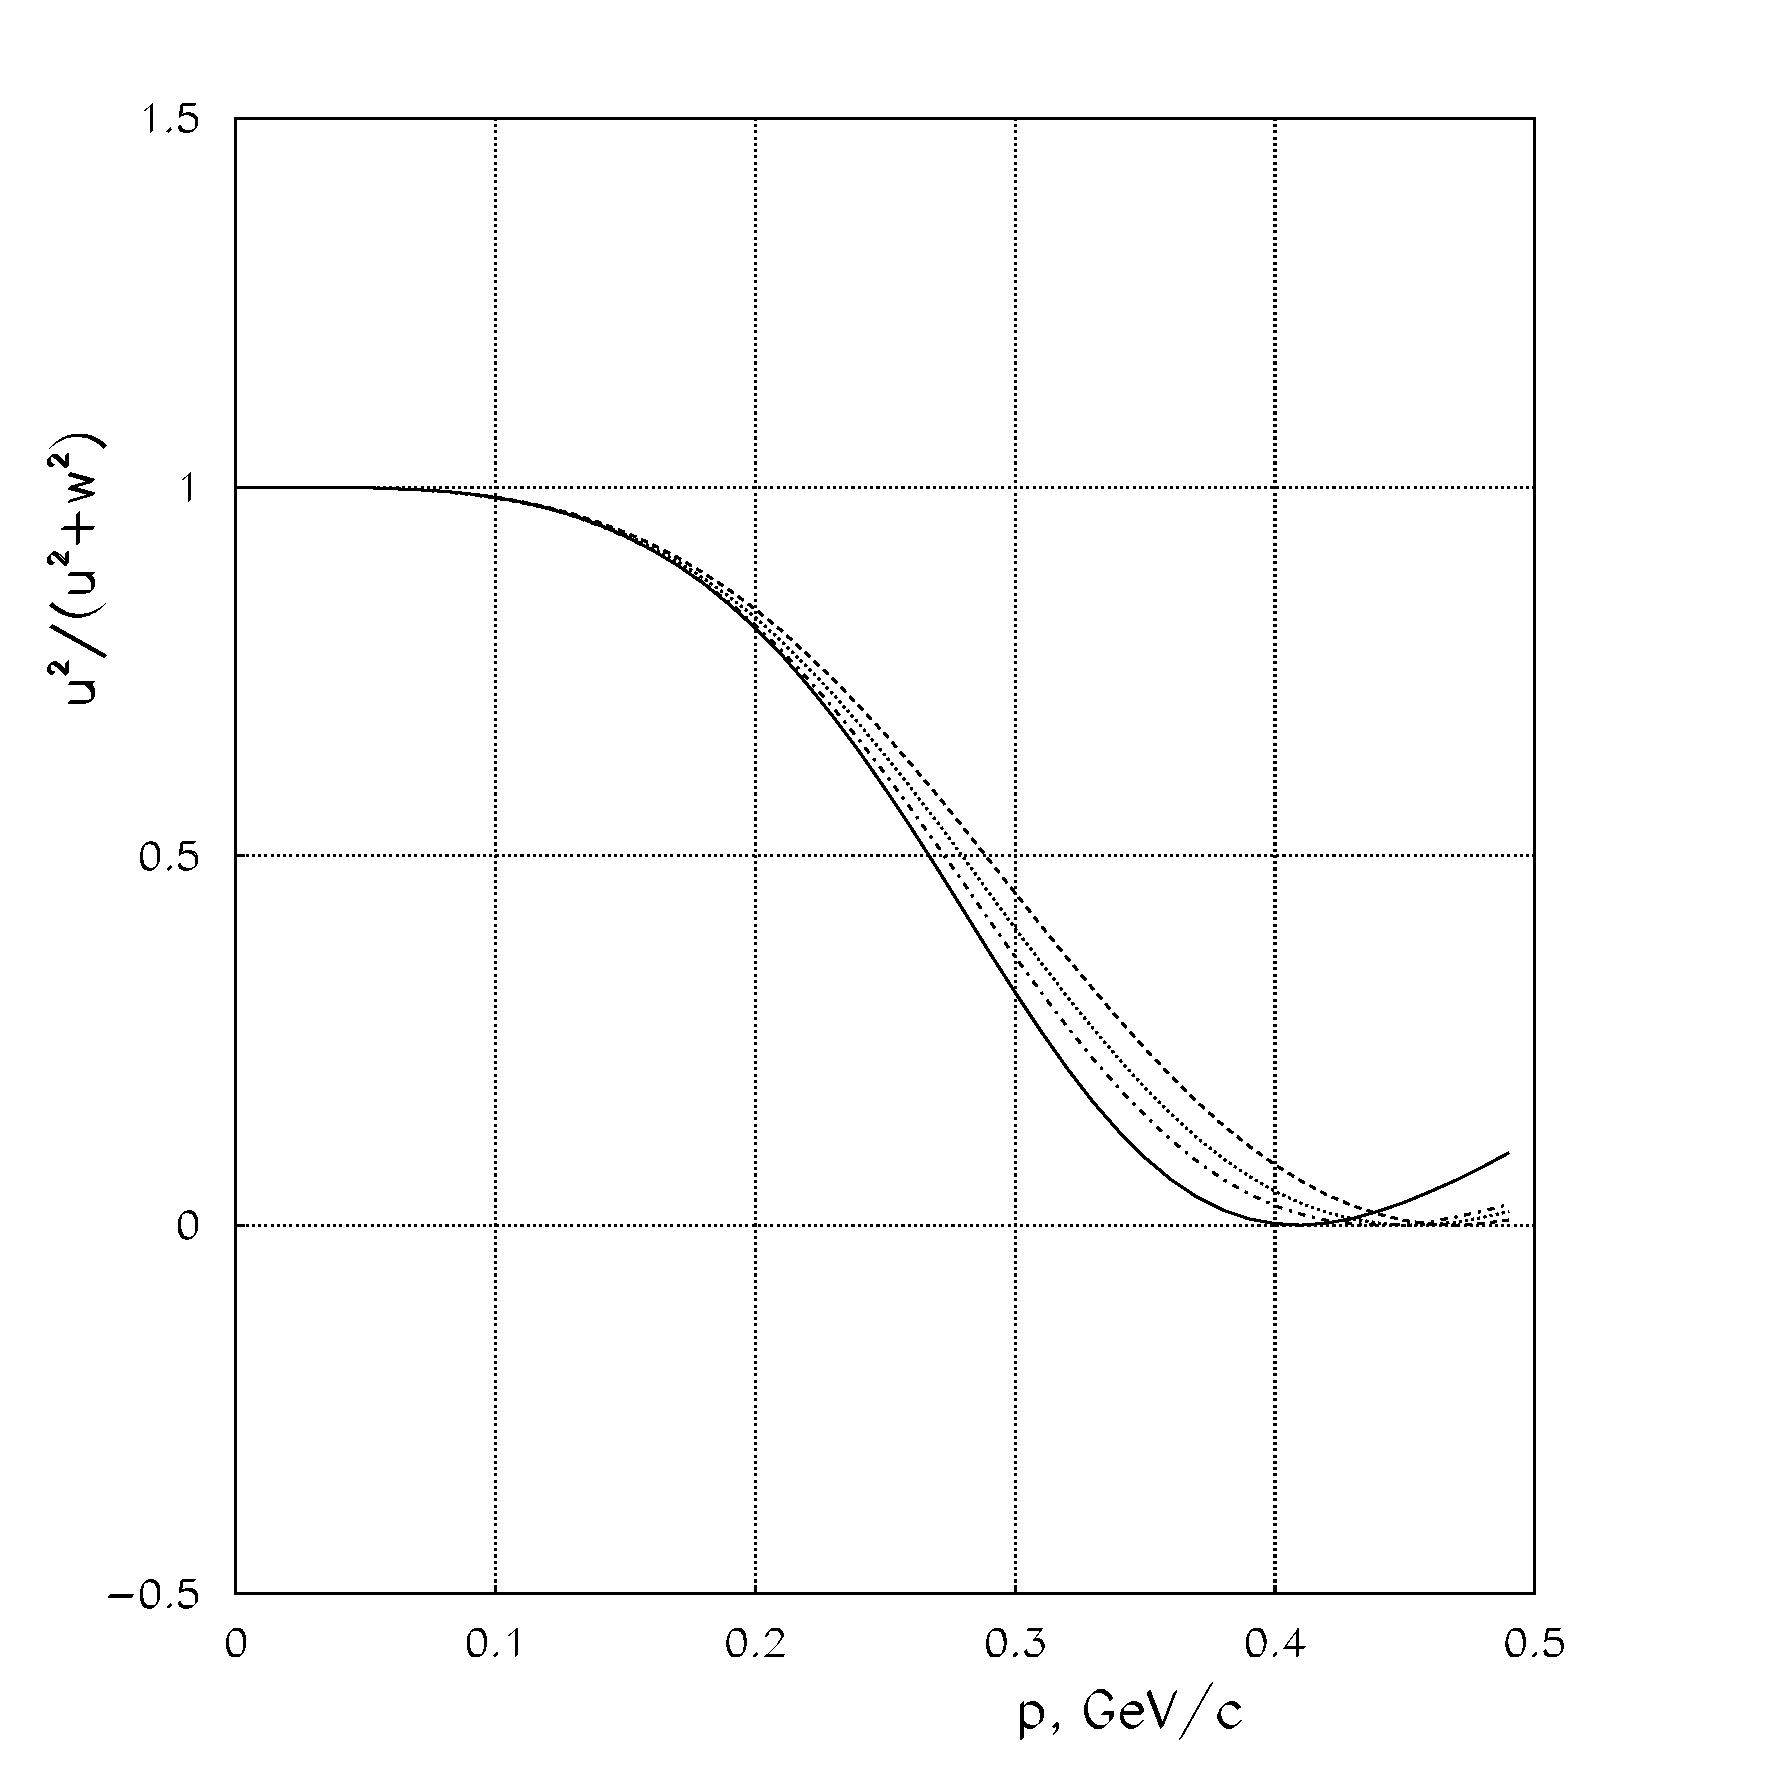
\includegraphics[width=10cm]{wavedtr.pdf}
        %\mbox{\epsfig{figure=wavedtr.eps,width=8.cm}}
      \end{center}
      \vspace{0.4mm}
      Рис.2  Вероятность S-волны как функция Ферми-импульса.
    \end{figure}

    \vspace {7mm}

    Оба указанные условия могут быть выполнены одновременно,
    если отбираются в лабораторной системе координат (быстрый
    протон падает на протонную мишень) события, содержащие два
    протона с импульсами близкими к половине импульса дейтрона
    в узком угловом конусе. Необхо\-димо отметить, что такая задача
    может быть успешно реализована только в пучках ускоренных
    дейтронов. В случае дейтериевой мишени оба протона слишком
    медленные, чтобы быть детектируемыми, а реакция идентифицирована.
    Чтобы ответить на вопрос о вкладе поворота
    спина в np$\to$pn процессе, как следует из выражения (2),
    необхо\-димы данные по дифференциальному сечению np$\to$pn
    перезарядки при t=0. Такие данные были получены в
    Брукхейвене~\cite{Fri}   для области 1-8 ГэВ и могли быть разумно
    аппроксимированы функцией $^1/p^2$, где p-импульс \hspace{0.1cm}
    падающе\-го нейтрона. При 1.67 ГэВ/c получено значение
    $\frac{d\sigma}{dt} (0)=(36,9\pm3,0)(ГэВ/c)^2$.
    Задача состоит в сравнении дифференциального сечения
    перезарядки на дейтроне при t=0 с величиной такого сечения для
    np$\to$pn процесса при соответствующей энергии.

    \vspace {10mm}

    \newpage
        {\Large\bf 2. Эксперимент на водородной пузырьковой камере.}

        \vspace {10mm}

        Первые экспериментальные данные были получены на
        1-м жидко\-водородной пузырьковой камере ОИЯИ~\cite{gla,ala}
        в полной пространственной геометрии при 3,35 ГэВ/с.
        Использование пучков ядер, падающих на протонную мишень, делает
        все фрагменты ядер быстрыми в лабораторной системе координат
        и потому они могут быть детектированы, хорошо измерены и
        идентифицированы практически без потерь.
        С другой стороны, почти все потери из-за порога определения
        импульса в камере сосредото\-чены в упругом канале.
        Эти условия позво\-ляют изучать реакции, содер\-жащие не более
        одной нейтральной частицы в эксклюзивном подходе.

        Реакция dp$\to$ppn может быть разделена на два
        канала:

        \vspace {8mm}
        1. прямой канал, когда протон является самой быстрой частицей
        в системе покоя дейтрона и

        \vspace {8mm}
        2. перезарядку, когда самой быстрой частицей в системе покоя
        дейтрона является нейтрон.

        \vspace {10mm}
        Разделение этих двух каналов проиллюстрировано на рис.3, показы\-
        вающем распределение по квадрату четырехмерного переданного
        импуль\-са от налетающего протона к вторичному нейтрону.
        Определенная таким образом величина не зависит от конечного
        состояния, является ли он спектатором или участником реакции
        (не чувствительна к интерференции протонов). Заштрихованная часть
        на рис.3 соответствует каналу переза\-рядки dp$\to$(pp)n.

        % ******* Figure 2 *********
        \begin{figure}[hbt]
          \begin{center}
            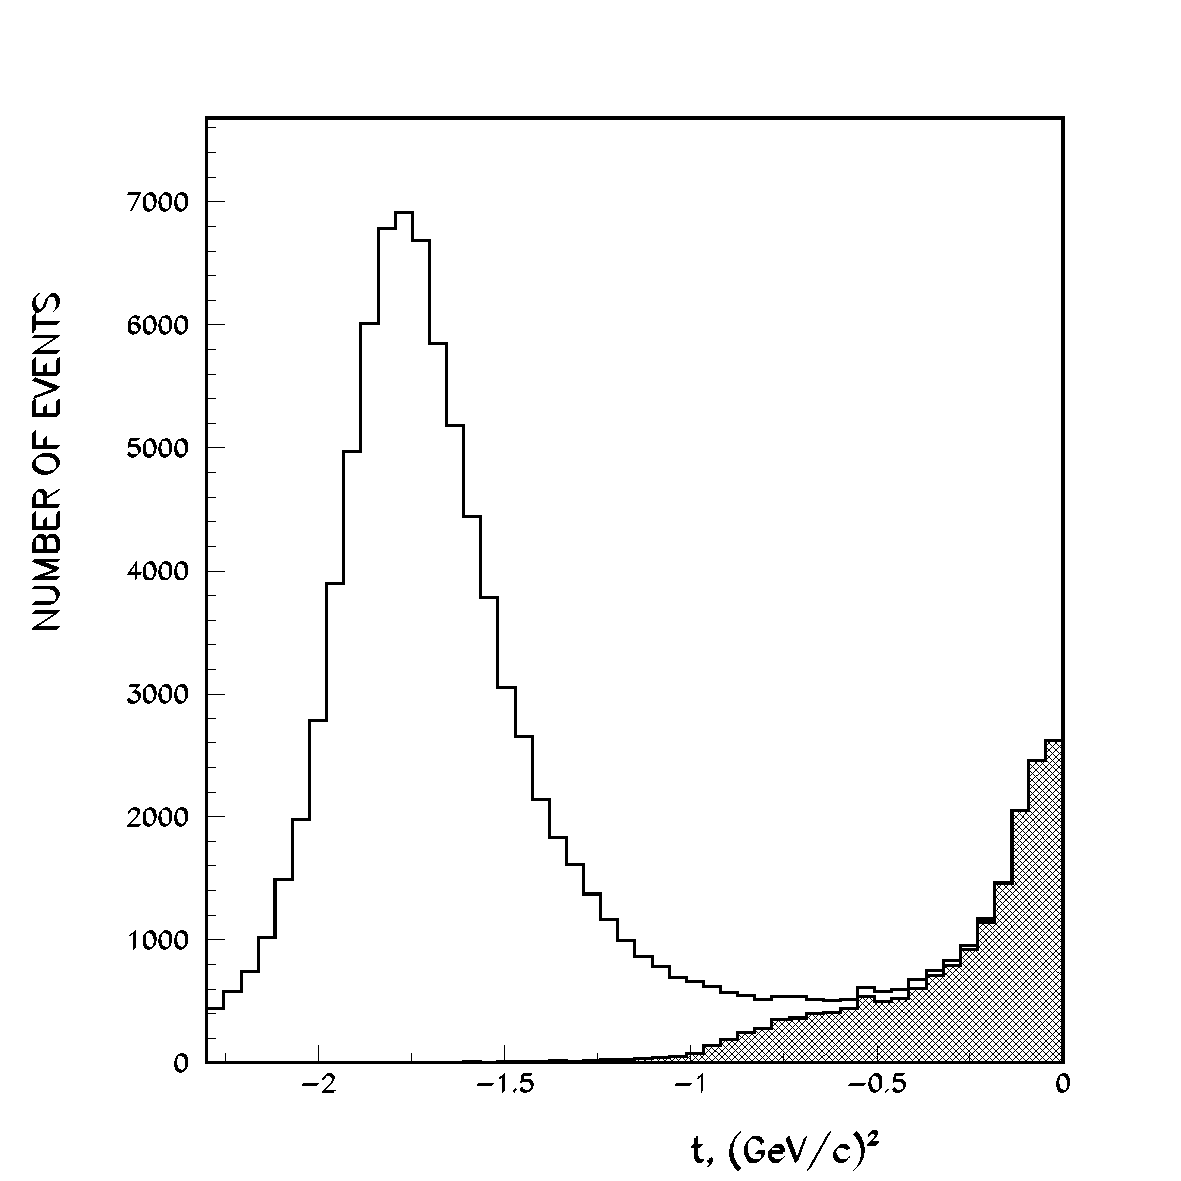
\includegraphics[width=8cm]{dist.pdf}
            %\mbox{\epsfig{figure=dist.eps,width=8.cm}}
          \end{center}
          \vspace{0.4mm}
          Рис. 3 Распределение по квадрату четырехмерного переданного
          импульса от мишени-протона к нейтрону.
        \end{figure}

        Для разумной интерполяции $\frac{d\sigma}{dt}$ к t=0
        важно выбрать область углов вылета протонов,
        исключающую высокоимпульсную часть внутреннего
        движения нуклонов, а также область передач импульса, где вступают
        в игру другие, более сложные, чем квазиупругое рассеяние механизмы.

        Дифференциальные поперечные сечения для четырех различных
        значе\-ний угла вылета обоих отобранных протонов показаны
        на рис. 4. Острота распределений при малых $\vert t\vert$
        не меняется с увеличением угла, тогда как вклад больших
        $\vert t\vert$ растет. Типичной величиной угла рождения является
        $\theta=arctg(P_f/P_0)=~1,6^0$, где экспериментальный
        и теоретический максимумы (pf=50 МэВ/с) распределения
        Ферми-импульсов нуклонов в дейтроне взят как измеренный поперечный
        импульс, а продольный импульс на нуклон в~лабораторной системе
        координат P$_0$ =1,67 ГэВ/с. Это дает оптимальную величину
        раскрытия конуса, в котором влетают оба протона около 3$^0$.

        % ******* Figure 2 *********
        \begin{figure}[hbt]
          \begin{center}
            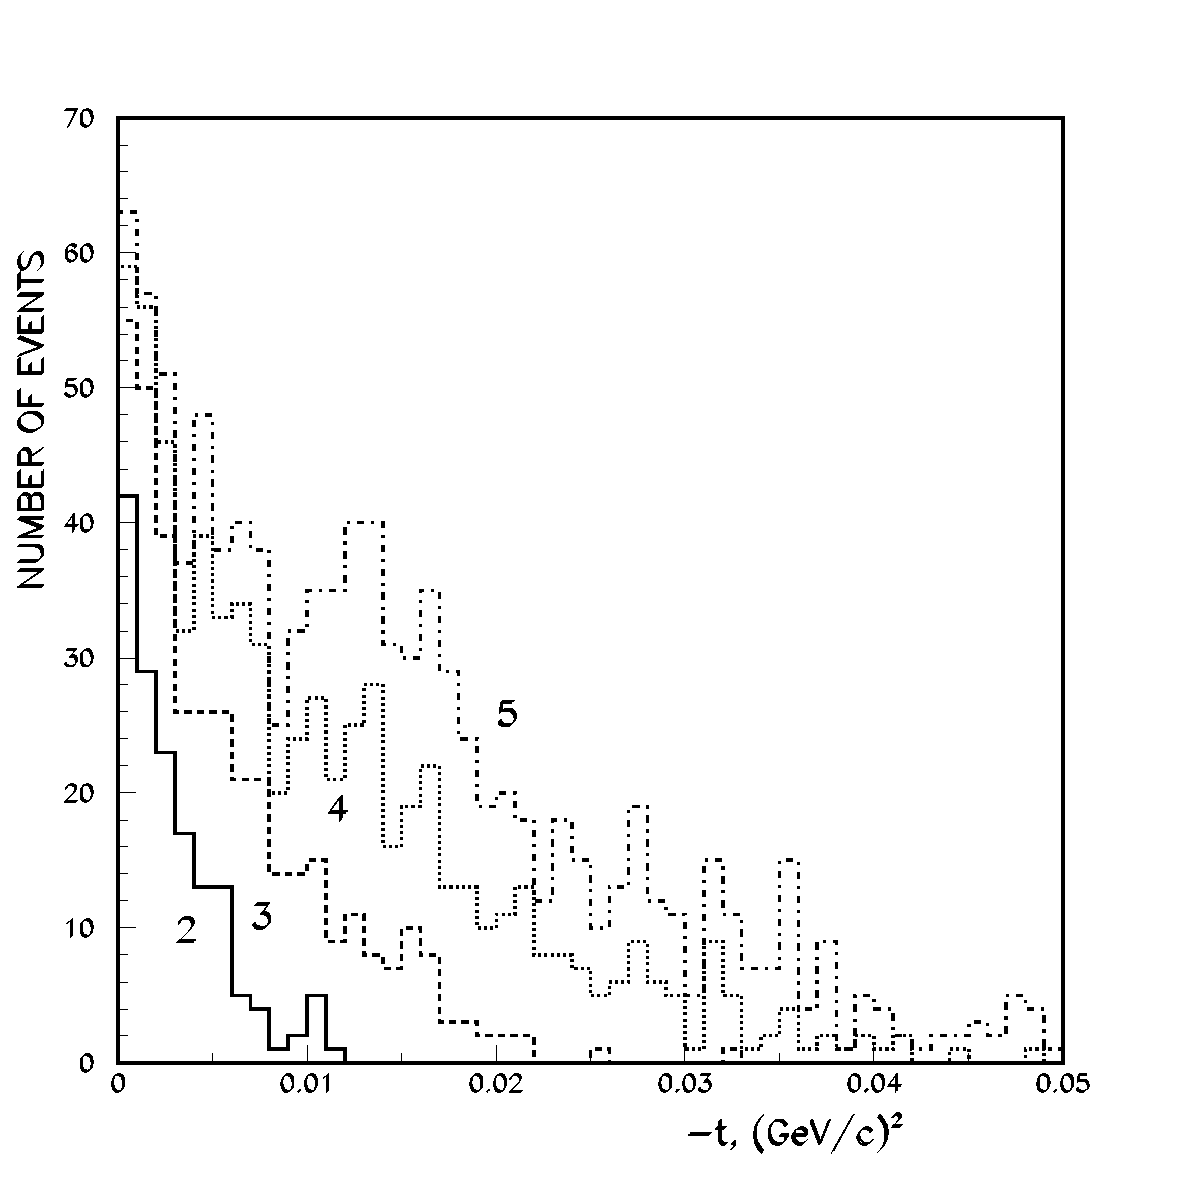
\includegraphics[width=8cm]{tpp2345.pdf}
            %\mbox{\epsfig{figure=tpp2345.eps,width=8.cm}}
          \end{center}
          \vspace{0.4mm}
          Рис. 4 Распределения по $\vert t\vert$ для канала перезарядки
          с углом вылета обоих протонов до 2, 3, 4 и 5 градусов. \\
        \end{figure}

        Рисунок 5 демонстрирует дифференциальное поперечное сечение реак\-ции
        перезарядки в функции угла отбора вылета двух протонов.
        Видно, что в районе $\theta$ =3$^0$ величина
        $\frac{d\sigma}{dt}$(0)
        достигает уровня $\frac{2}{3}\frac{d\sigma}{dt}$(0)
        для элемен\-тарной np$\to$pn перезарядки. Для $\theta$ =3$^0$
        мы оценили вклад части с поворотом спина в np$\to$pn процессе
        как 0,94$\pm$ 0,15.

        % ******* Figure 2 *********
        \begin{figure}[hbt]
          \begin{center}
            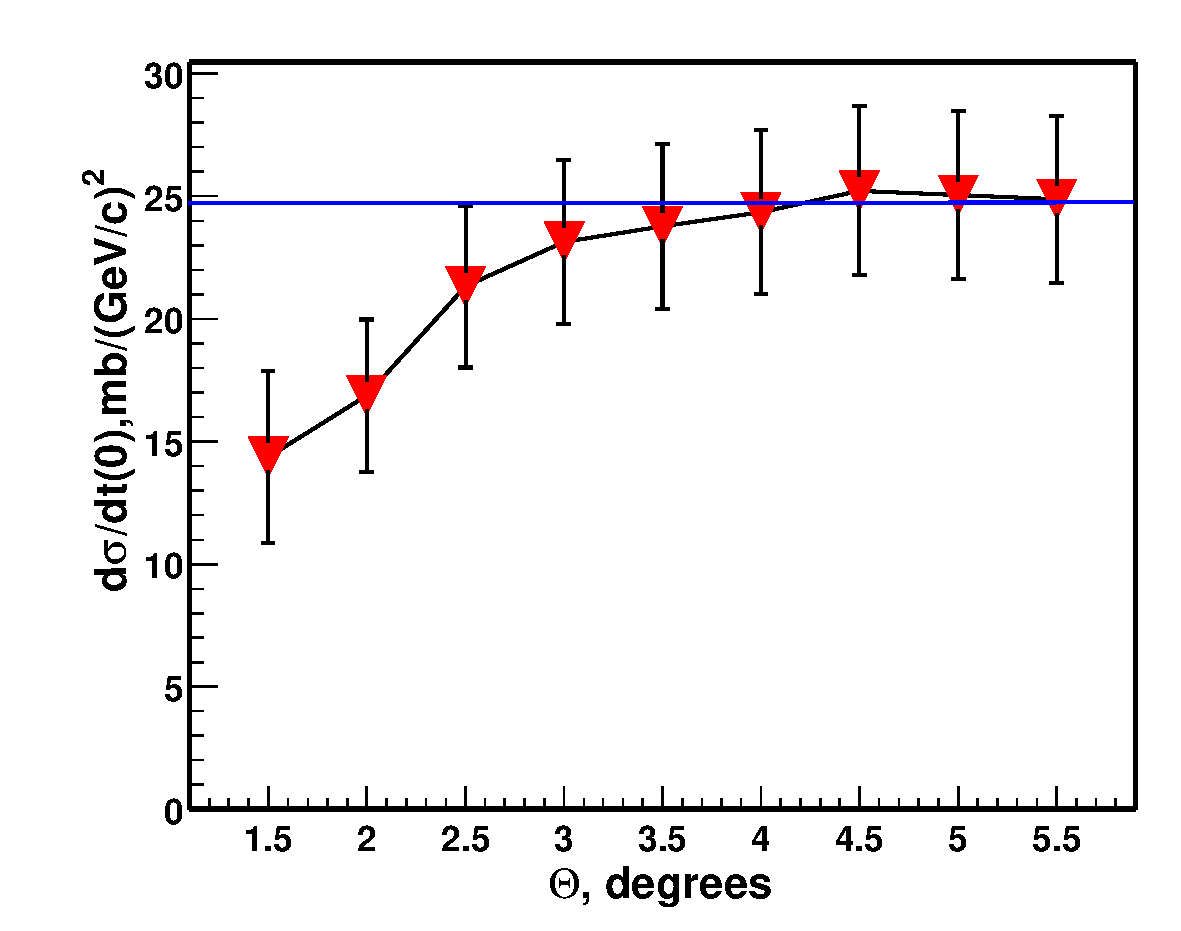
\includegraphics[width=9cm]{sigma0.pdf}
            %\mbox{\epsfig{figure=sigma0.eps,width=8.cm}}
          \end{center}
          \vspace{0.4mm}
          Рис. 5 Дифференциальное поперечное сечение при t=0 в случае
          когда оба протона вылетают в пределах угла $\theta$. \\
        \end{figure}

        Полученное значение зависит, конечно, от неизвестных систематических
        ошибок для дифференциального поперечного сечения элементарной
        np$\to$pn перезарядки. В любом случае, полученный вклад достаточно
        большой и не исключает полного поворота спина
        в np$\to$pn процессе. Это означает, что при работе
        в пучках векторно поляризованных протонов
        можно получить дополнительные возможности
        использования изучаемой реакции для более расширенных целей,
        т.е. например для объяснения механизма интерферен\-ции в системе
        двух протонов. Спектатор и рас\-сеянный протон помечены,
        т. к. один из них сохраняет поляризацию пучка, а второй (рассеянный)
        поляризован противоположно.

        \vspace {10mm}
        \newpage

        {\Large \bf 3. Новая установка СТРЕЛА.}

        \vspace {10mm}
        Геометрия, детекторы и фоновые условия были оценены на основе:

        \vspace {8mm}
        1) генерации Монте Карло

        \vspace {8mm}
        2) реальных событий из 17 различных dp-реакций.

        \vspace {10mm}
        В качестве исходных были использованы следующие параметры:
        сече\-ние пучка в области мишени-1 см; импульс пучка 3,5 ГэВ/c;
        толщина жидко\-водородной мишени 10 см; длина полюса магнита-1 м.
        и поле -1Т; расстояние от мишени до магнита 1м и до первого
        из детекторов телескопа 7 м; поперечный размер детектора 5 см.
        При расчетах исполь\-зовалась волновая функция
        Гартенхаузер-Мо\-равчика и экспериментальные наклоны
        дифференциальных сечений Nd и NN упругого рассеяния.

        Указанные параметры могли быть оптимизированы согласно
        требова\-ний к геометрии установки.

        Экспериментальные и Монте Карло оценки фона от одно-протонных
        событий, т. е. от прямого развала дейтрона дали примерно одинаковые
        результаты. Ожидается не более 400 однопротонных событий на одно
        двухпротонное при апертуре отбора 0,5$^0$. Отношение эффект-фон
        улуч\-шается при увеличении этого угла. В случае однопротонных
        событий детекти\-руемые протоны является в основном спектаторами,
        что дает основу для норми\-ровки сечений.

        Итак, должны быть зарегистрированы два протона, каждый с импуль\-сом
        в половину импульса падающего дейтрона. Это значит, что отби\-раются
        события под 0$^0$ по отношению к направлению пучка с малым
        относитель\-ным импульсом внутрен\-него движения в дейтроне и малым
        переданным к рассеянному нейтрону импульсом.

        Тем самым возможно реализовать минимально необходимые условия
        для регистрации предполагаемого эффекта.
        В качестве первой стадии предложена экспериментальная схема,
        показанная на рис. 6.

        % ******* Figure 2 *********
        \begin{figure}[hbt]
          \begin{center}
            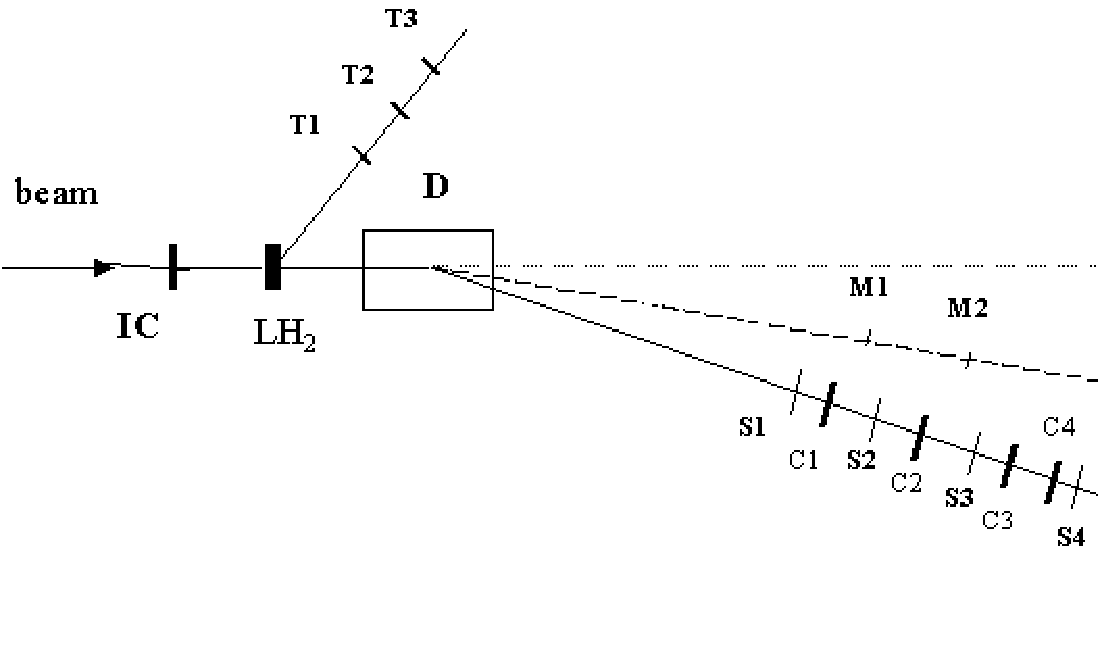
\includegraphics[width=9cm]{image2.pdf}
            %\mbox{\epsfig{figure=Image2.eps,width=8.cm}}
          \end{center}
          \vspace{0.4mm}
          Рис. 6 Схема экспериментальной установки. \\
        \end{figure}

        Выведенный дейтронный пучок падает на 10 см. жидководородную
        мишень LH$_2$ и анализирующий магнит D разделяет первичные
        дейтроны и вторичные частицы. Иони\-зационная камера IC измеряет
        поток дейтро\-нов пучка. Сцин\-тилляционные мониторы Т1-Т3 и М1-М2
        контролируют интенсивность и положение пучка.
        Сцинтилляционные счетчики S1-S4 диаметром 48 мм определяют
        угловой и импульсный (10\%) аксептансы и триггируют события.
        Черенковские счетчики С1-С3 с полистироловыми радиаторами
        размера 50*50*16мм$^3$ отбирают двухпротонные события.
        Ожидаемое разрешение около 10\% позволяет реально разделить
        одно и двухпротонные события.Черенковский счетчик С4 с кварцевым
        радиато\-ром служит для подавления пионов. Амплитуды сигналов со всех
        счетчиков записываются для каждого триггируемого события. Чтобы
        сделать отбор событий более эффективным, предусмотрена возможность
        вклю\-чения в логический триггер амплитудного сигнала с одного
        из Черенков\-ских счетчиков.

        \vspace {10mm}

        {\Large\bf 4. Планирование измерений и первая проба
          установки СТРЕЛА.}

        \vspace {10mm}

        При угловом аксептансе 5*10$^{-2}$ мстр и импульсном аксептансе 5\%
        пред\-полагается получить при каж\-дой из энергий, указанных
        в таблице до 2000 двухпротонных событий при интенсивности
        10$^7$ дейтронов в сбросе из ускорителя. В каждой точке необходима
        подстройка Нуклотрона и дополнительное время для контроля детекторов
        и параметров пучка, что не включено в последнюю колонку таблицы.

        \begin{tabular}{|c|c|c|c|c|c|}    \hline
          N    &  Td (GeV)&       Deuteron & One proton & Two proton & Time \\
          & &        momentum  & event  & events  & (min) \\
          & &(GeV/c)&     &       &       \\ \hline
          1   &   1.41 &  2.7  &  3100 &  8  &    50 \\  \hline
          2   &   1.49 &  2.8  &  3100 &  8  &    50 \\  \hline
          3   &   1.58 &  2.9  &  3100 &  8  &    50 \\  \hline
          4   &   1.66 &  3.0  &  3200 &  9  &    50 \\  \hline
          5   &   1.75 &  3.1  &  3200 &  9  &    50 \\  \hline
          6   &   1.83 &  3.2  &  3300 &  10 &    40 \\  \hline
          7   &   1.92 &  3.3 &   3400 &  10 &    40 \\  \hline
          8   &   2.00 &  3.4 &   3600 &  10 &    40 \\  \hline
          9   &   2.09 &  3.5 &   3800 &  11 &    40 \\  \hline
          10  &   2.18 &  3.6 &   4200 &  11 &    40 \\  \hline
          11  &   2.27 &  3.7 &   4400 &  12 &    40 \\  \hline
          12  &   2.36 &  3.8 &   4800 &  13 &    30 \\  \hline
          13  &   2.45 &  3.9 &   5100 &  14 &    30 \\  \hline
          14  &   2.54 &  4.0 &   5400 &  15 &    30 \\  \hline
        \end{tabular}
        \vspace*{5mm}

        В марте 2000 года был проведен первый сеанс установки СТРЕЛА
        показаны принципиальные возможности юстировки телескопа на
        максимум стриппинга дейтронов (рис. 7) и отбора двухпротонных
        событий (рис. 8).

        % ******* Figure 2 *********
        \begin{figure}[hbt]
          \begin{center}
            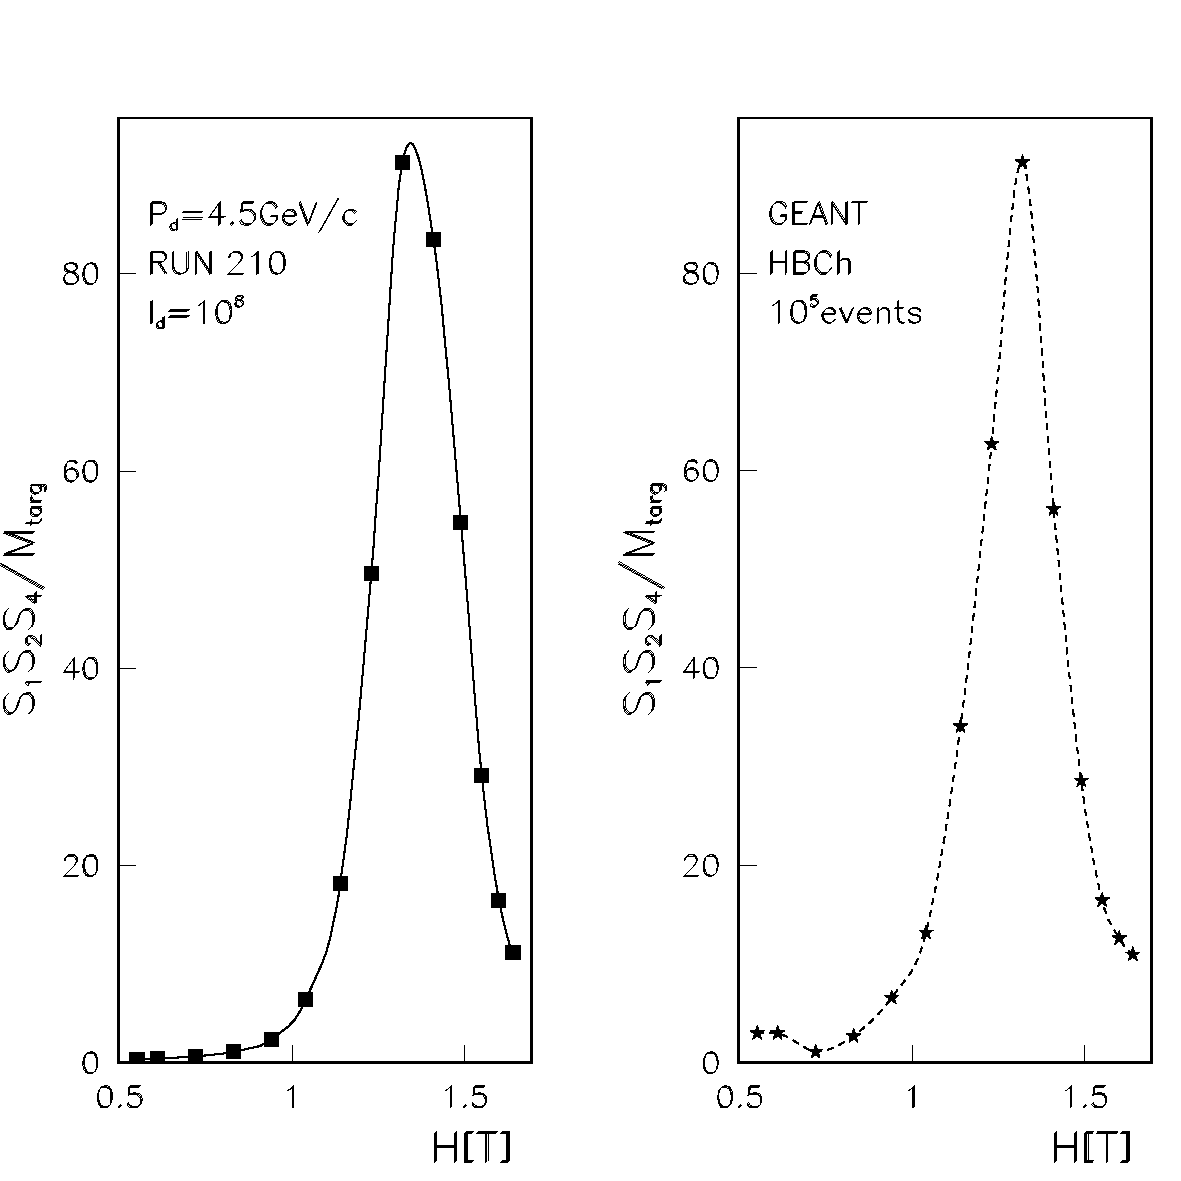
\includegraphics[width=8cm]{s3ok.pdf}
            %\mbox{\epsfig{figure=s3ok.eps,width=8.cm}}
          \end{center}
          \vspace{0.4mm}
          Рис. 7  Экспериментальное и Монте-Карло распределения протонов
          стриппинга.
        \end{figure}

        % ******* Figure 2 *********
        \begin{figure}[hbt]
          \begin{center}
            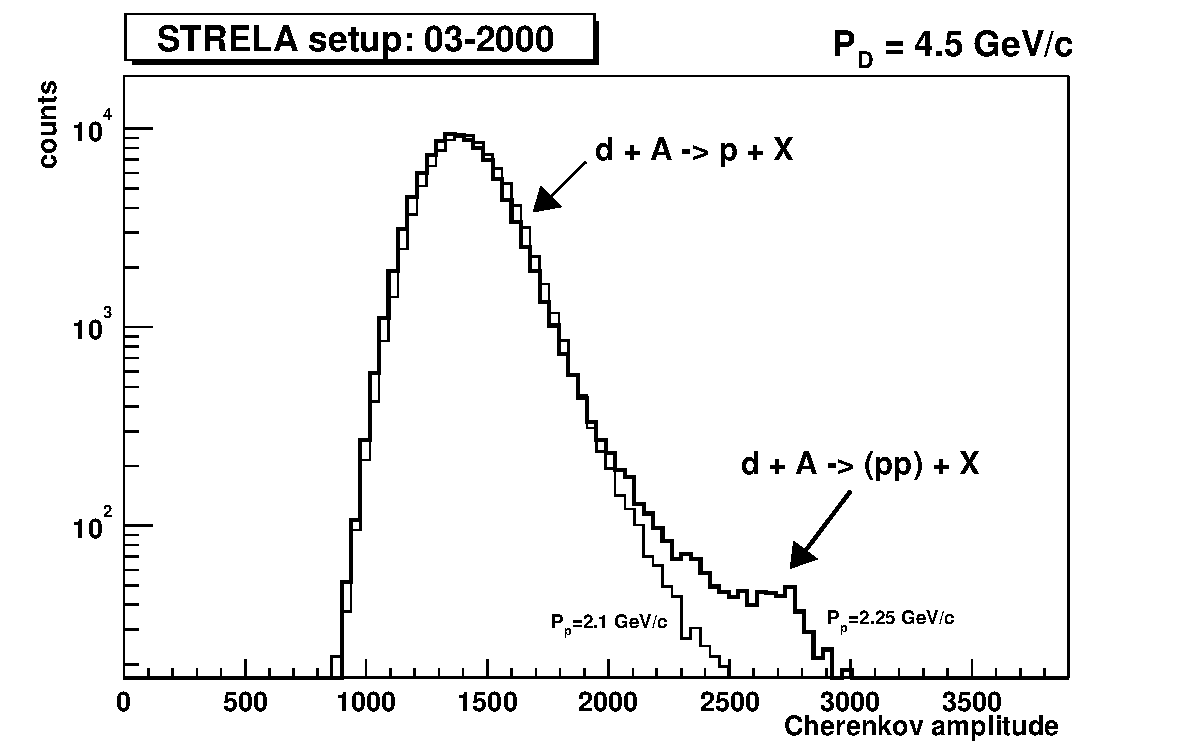
\includegraphics[width=8cm]{strela.pdf}
            %\mbox{\epsfig{figure=strela.eps,width=8.cm}}
          \end{center}
          \vspace{0.4mm}
          Рис. 8  Черенковские амплитуды для одно и двухпротонных событий \\
        \end{figure}

        \begin {thebibliography}{999}

          \addcontentsline{toc}{chapter}{\bibname}
        \bibitem{Mig} А.Б.Мигдал,//ЖЭТФ 28,1955 г.,стр.3.
        \bibitem{Pom} И.Померанчук,//ДАН СССР,1951 г.,т.LXXVIII,№2,стр.249.
        \bibitem{Dea} N.W.Dean,//Phys.Rev.D5,1972,p.461.
        \bibitem{Fri} J.L.Friedes et al.//Phys.Rev.Lett 15,1965,pp.38-41.
        \bibitem{gla} V.V. Glagolev, Nucl.Phys. B (proc.Suppl.) 36 (1994) 509-512
        \bibitem{ala} B.S.Aladashvili et al. //Nucl.Phys.B86, 1975, p.461.
        \end{thebibliography}

\end{document}
